\subsection*{Updated Data Flow Diagrams}

\subsubsection*{Level 0 DFD}

Here is our updated top level DFD:

\begin{center}
  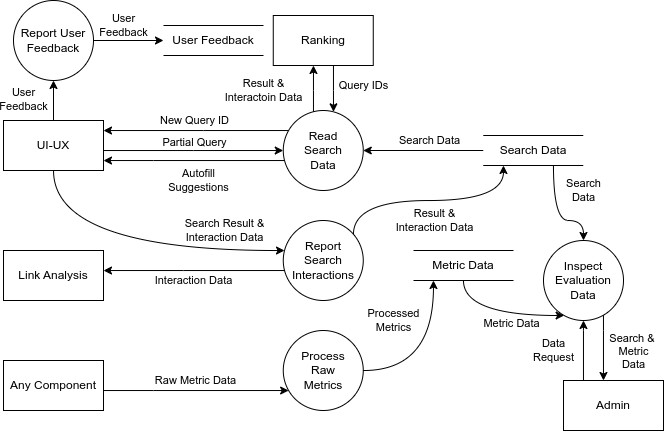
\includegraphics[scale=0.5]{DFDs/HighLevelDFD.drawio (1).png}
\end{center}
High Level Changes:
\begin{itemize}
  \item Ranking now asks for interaction data instead of us sending it to them on each query
  \item Added the Report User Feedback process for UI/UX
  \item Condensed read operations into one high level process
\end{itemize}

Report User Feedback is a simple operation, so no lower level DFDs are needed. The exact data received form UI/UX will be dumped to text files.

\subsubsection*{Level 1 DFDs}

\textbf{Read Search Data}

\medskip

Both the Ranking and UI/UX components will need to read data from our database in one way or another. UI/UX will need autofill suggestions and unique query IDs. Neither of these are directly stored, the way the interaction data that Ranking needs is, but they will still rely on the database contents to do this.

\begin{center}
  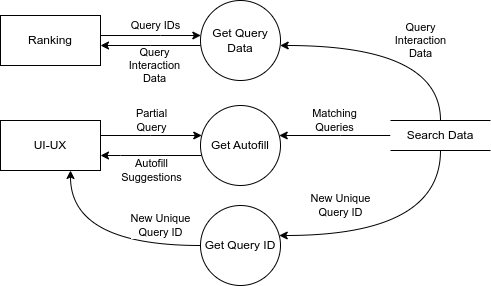
\includegraphics[scale=0.5]{DFDs/LowLevelDFDs-ReadSearchData.drawio.png}
\end{center}

\textbf{Report Search Interactions}

\medskip

After each query, the UI/UX team will send the user interaction data to us to be stored. Certain data will also be forwarded to Link Analysis for updating of the web-graph.

\begin{center}
  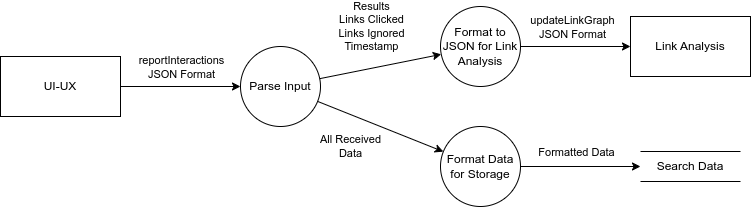
\includegraphics[scale=0.5]{DFDs/LowLevelDFDs-ReportSearchResults.drawio (2).png}
\end{center}
\subsection*{Functional Decomposition Diagrams}

\textbf{Process Raw Metrics}

\medskip

All components will be sending metrics data periodically. This will be in a variety of formats, but will be aggregated together for storage in the Metric Data Database.

\begin{center}
  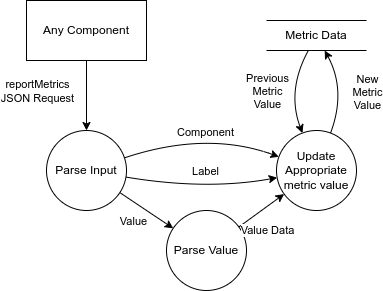
\includegraphics[scale=0.5]{DFDs/LowLevelDFDs-ReportMetric.drawio (1).png}
\end{center}

\textbf{Inspect Evaluation Data}

\medskip

The system administrator will have the opportunity to interact with our component through a command line interface to inspect the logged search history as well as the performance metrics. 

\begin{center}
  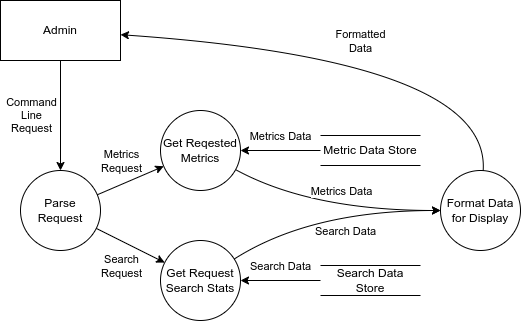
\includegraphics[scale=0.5]{DFDs/LowLevelDFDs-AdminView.drawio (1).png}
\end{center}

\subsubsection*{Level 2 DFD}

\textbf{Get Autofill}

\medskip

The other level 1 processes are relatively trivial, however autofill deserves a further expansion. We will attempt to correct typos, and search for similar queries (with and without typos). They will then be ranked and sent back to UI/UX.

\begin{center}
  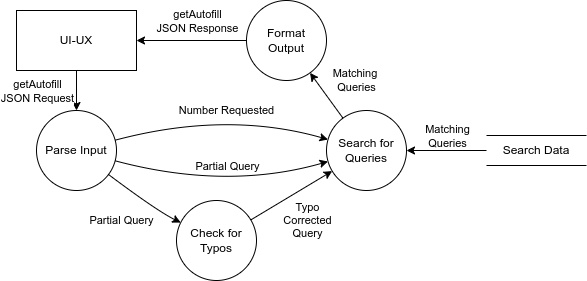
\includegraphics[scale=0.5]{DFDs/LowLevelDFDs-GetAutofill.drawio (2).png}
\end{center}

\subsection*{Architectural Divisions}